\documentclass[10pt]{beamer}

\usetheme{Madrid}
\usepackage[utf8]{inputenc}
\usepackage[english]{babel}
\usepackage{amsmath}
\usepackage{amsfonts}
\usepackage{amssymb}
\usepackage{graphicx}
\usepackage{ragged2e}
\usepackage{booktabs}
\usepackage{hyperref}
\usepackage{float}
\usepackage[T1]{fontenc}
\usepackage{changepage}
\usepackage{tikz}
%para enumerar tablas y figuras
\usepackage{caption}
\setbeamertemplate{caption}[numbered]

%\setbeamertemplate{bibliography item}[text]
\addtobeamertemplate{title page}{\centering 
\includegraphics[scale=0.40]{figuras/logo11}\\}

\title[The Miracle of Microfinance?]{The Miracle of Microfinance? Evidence from a Randomized Evaluation\\}
\author[Experimental Economics]{
{\small{Banerjee, A., Duflo, E., Glennerster, R. and Kinnan, C.}\\[0.6cm]}
Group 1:\\
Sebastián Solano, Benjamín Solis, Matías Vicuña and Rodrigo Jiménez\\[0.2cm]
\small{Professor: Ricardo Barros}\\
\small{Experimental economics}\\
}
\institute[\tiny{U. Javeriana}]{}
\date[\tiny{November 2024}]{\footnotesize{November 2024}}
% Incluir el logo en la esquina superior derecha, sobre la franja azul
\addtobeamertemplate{frametitle}{}{%
    \begin{tikzpicture}[remember picture, overlay]
        \node[anchor=north east, yshift=3pt, xshift=-4pt] at (current page.north east) 
            {
\includegraphics[scale=0.15]{figuras/logo12}};
    \end{tikzpicture}%
}
%\setbeamercovered{transparent}
%\setbeamertemplate{navigation symbols}{} 
%\date{} 
%\subject{}


\begin{document}
%%para que aparezca tabla en vez de cuadro
%\renewcommand{\listtablename}{Índice de tablas}
%\renewcommand{\tablename}{Tabla}

\begin{frame}[plain,t]
\titlepage
\end{frame}

%\begin{frame}{Contenido}
%\tableofcontents
%\end{frame}

\section{introduction}
\begin{frame}{Introduction}
\justifying
\textbf{Publication}: \cite{banerjee2015} article in the journal American Economic.\\
\vspace{\baselineskip}
\textbf{Objective}:. Evaluation of a group microcredit program targeting women who are not necessarily entrepreneurs.\\
\vspace{\baselineskip}
\textbf{Location}: Hyderabad, India (52 randomly selected neighborhoods).\\
\vspace{\baselineskip}
\textbf{Relevant results}
\begin{itemize}
    \justifying
    \item Increase in Microcredits: 8.4 percentage point increase in microloan uptake.
\end{itemize}
\textbf{Institutions Involved}
\begin{itemize}
    \item Centre for Micro Finance (CMF), IFMR, Chennai.\\
    \item Spandana: Fast-growing microfinance institution. 
\end{itemize}
\textbf{Areas Evaluated}
\begin{itemize}
\item Consumption, business start-ups, business income.\\
\item Human development: Education, health, women's empowerment.
\end{itemize}
\end{frame}

\section{motivation}
\begin{frame}{Motivation}
\justifying
\textbf{Rapid Expansion:} Last 10 to 15 years.\\
\textbf{Global Impact:}
\begin{itemize}
\item Increase in families benefiting from microcredit.\\
\item From 7.6 million in 1997 to 137.5 million in 2010 (Microcredit Summit, 2012).
\end{itemize}

\textbf{Microcredit and Poverty Reduction}
\begin{itemize}
    \justifying
    \item Poverty Alleviation Expectation: Generates hope for rapid poverty reduction.\\
\item International Recognition: Nobel Peace Prize (2006) awarded to Mohammed Yunus and Grameen Bank for their contribution to global poverty reduction.
\end{itemize}

\begin{figure}[H]
\centering
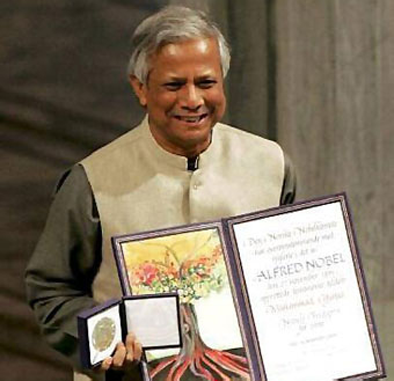
\includegraphics[scale=0.2]{figuras/yunus_nobel_01}
{\footnotesize
\caption{Muhammad Yunus. Source: Biografiasyvidas.}
}
\label{figura02}
\end{figure}

\end{frame}

\begin{frame}{Motivation}
\justifying
\textbf{Critical Information on Microcredit: New York Times article:}
\begin{itemize}
\item Relating to suicides due to over-indebtedness.\\
\item Reddy Subrahmanyam (Andhra Pradesh) accuses MFIs of making “hyper-profits at the expense of the poor”.
\end{itemize}
\vspace{\baselineskip}
\textbf{Misleading anecdotes:} Stories of success or over-indebtedness do not reflect the effect on the average borrower.\\
\textbf{Insufficient representative data:} They do not allow identifying the causal effect of access to microfinance, as clients are self-selected.\\
\textbf{Choice of locations:} MFIs choose certain towns to operate in, complicating evaluation.\\
\vspace{\baselineskip}
\textbf{First randomized evaluation:}
\begin{itemize}
    \justifying
    \item Analyzes group microcredit model targeting women not necessarily entrepreneurs.\\
\item Follow-up of households for 3 to 3.5 years, necessary to detect medium-term impacts.
\end{itemize}

\end{frame}
	
\section{Data mining}
\begin{frame}{Data source}
        \justifying
        Los datos utilizados incluyen los precios de cierre diarios de los siguientes activos financieros: COPEC, ENTEL, Falabella, CMPC, Aesandes (Gener), Besalco, Watts y SALMOCAM, además de los índices IPSA e IGPA, desde enero de 2018 a diciembre de 2023. \textbf{Fuente:} Investing y Yahoo Finance.\\
        \vspace{\baselineskip} % Espacio adicional entre párrafos
        Los datos del Banco Central incluyen los bonos del Banco Central a 10 años en U.F. \textbf{Fuente:} Banco Central de Chile.
\end{frame}

\section{Methodology}
\begin{frame}{Methodology}
        \justifying
        Los datos utilizados deben tener como propiedad que la distribución de sus errores sea simétrica, para poder utilizar una distribución elíptica en el modelo.\\
        
\begin{figure}[H]
\centering
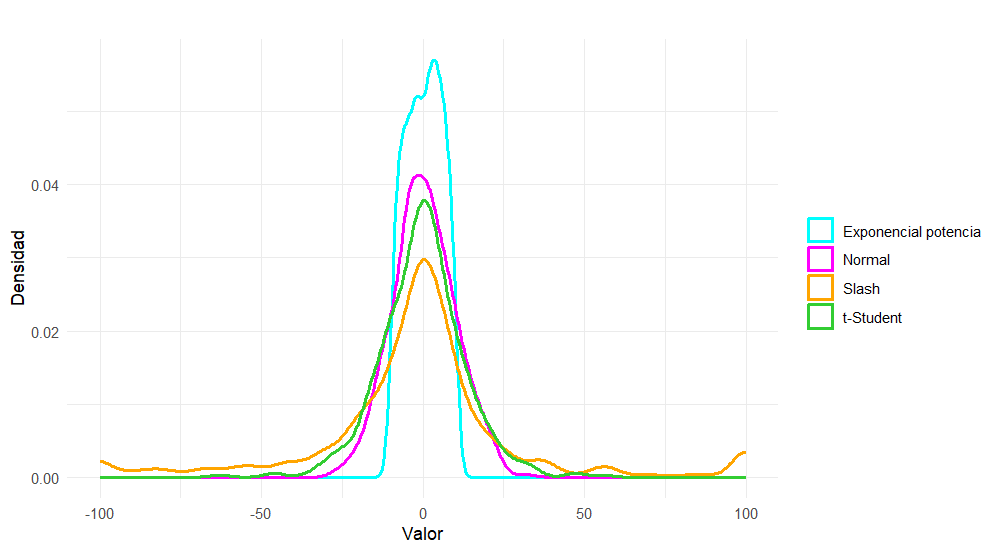
\includegraphics[scale=0.45]{figuras/FIGURA_02_01}
{\footnotesize
\caption{Comparativa densidad distribuciones elípticas. Fuente: Elaboración propia.}
}
\label{figura01}
\end{figure}
\end{frame}

\begin{frame}{Methodology}

\textbf{Lilliefors}
    \begin{equation}
    D_n = \max_{-\infty < x < \infty} \left| F_n(x) - F(x; \hat{\mu}, \hat{\sigma}^2) \right|
    \end{equation}
    donde:
    \begin{itemize}
        \item \( D_n \): Estadística de prueba del test de Lilliefors.
        
        \item \( F_n(x) \): La función de distribución empírica (FDE) de la muestra:
        \[
        F_n(x) = \frac{1}{n} \sum_{i=1}^{n} I(X_i \leq x)
        \]
        
        \item \( F(x; \hat{\mu}, \hat{\sigma}^2) \): La función de distribución normal con media \( \hat{\mu} \) y varianza \( \hat{\sigma}^2 \):
        \[
        F(x; \hat{\mu}, \hat{\sigma}^2) = \Phi\left( \frac{x - \hat{\mu}}{\hat{\sigma}} \right)
        \]
    \end{itemize}
\end{frame}

\section{Results}
\begin{frame}{Results}
    \centering
    \begin{table}[ht]
        \centering
        \begin{tabular}{c c}
            \toprule
            \textbf{\textit{Estadístico}} & \textbf{\textit{Valor}} \\ 
            \midrule
            \textit{Skewness (asimetría)} & \textit{0.30367} \\ 
            \textit{Estadístico Z}       & \textit{1.11600} \\ 
            \textit{p-value}             & \textit{0.2644} \\ 
            \textit{Hipótesis alternativa} & \textit{Datos tienen asimetría} \\ 
            \bottomrule
        \end{tabular}
        \caption{Test Asimetría de D'Agostino para Besalco. Fuente: Elaboración propia.}
    \end{table}
    
\begin{table}[ht]
\centering
\begin{tabular}{l c}
\toprule
\textbf{Estadístico} & \textbf{Valor} \\
\midrule
Chi-squared & 1.0913 \\
df       & 2       \\
p-value  & 0.5795 \\
\textit{Hipótesis alternativa} & \textit{Datos no provienen de una normal}\\
\bottomrule
\end{tabular}
\caption{Test de Jarque-Bera para Besalco. Fuente: Elaboración propia.}
\end{table}
\end{frame}

\begin{frame}{Graphics}
        \justifying
        Las siguientes figuras corresponden a gráficos de los retornos mensuales de Besalco basados en \textbf{precios de cierre diarios ajustados}.\\
        
\begin{figure}[H]
\centering
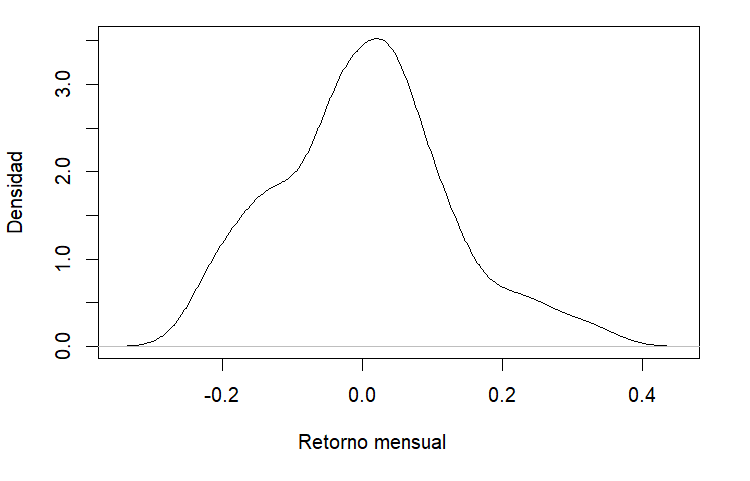
\includegraphics[scale=0.5]{figuras/FIGURA_02_03}
{\footnotesize
\caption{Densidad retornos Besalco (2018-2023). Fuente: Elaboración propia.}
}
\label{figura02}
\end{figure}
\end{frame}

\begin{frame}{Description table}
\begin{table}[ht]
        \centering
        \small % Cambia el tamaño del texto de la tabla
\begin{tabular}{l r}
\toprule
\textbf{\textit{Estadístico}} & \textbf{\textit{Valor}} \\
\midrule
\textit{Mínimo}             & -0.230746559   \\
\textit{Máximo}             & 0.334786499     \\
\textit{Rango}           & 0.565533059    \\
\textit{Mediana}          & 0.007561071     \\
\textit{Media}            & 0.002731092     \\
\textit{Error estándar de la media}         & 0.014518750 \\
\textit{IC media (95\%)}    & 0.028956733     \\
\textit{varianza}             & 0.014966381     \\
\textit{Desviación estándar}         & 0.122337160     \\
\textit{Coeficiente de variación}        & 44.794235570    \\
\textit{Asimetría}        & 0.297276866     \\
\textit{Curtosis}        & -0.078276872   \\
\textit{Shapiro-Wilk W}      & 0.980553143     \\
\textit{Valor p Shapiro-Wilk}      & 0.338553548     \\
\bottomrule
\end{tabular}
        \caption{Estadísticos descriptivos retornos Besalco. Fuente: Elaboración propia}
    \end{table}
\end{frame}

\section{Conclusions}
\begin{frame}{Conclusions}
\justifying
\textbf{Limited Demand:} Only 33\% of households apply for loans from an MFI at the end of a three-year study.\\
\vspace{\baselineskip}
\textbf{Business Impact:} Although some borrowers expand businesses, they do not escape poverty through microfinance.\\
\vspace{\baselineskip}
\textbf{General Welfare:} There is no increase in the monthly consumption of those who accessed microfinance, either in the short or long term.\\
\vspace{\baselineskip}
\textbf{Business Benefits:} Most companies do not see an increase in profits, although there are improvements in companies with high profitability.\\
\vspace{\baselineskip}
\textbf{Effect on Social Outcomes:} In Hyderabad, access to microcredit shows no effect on education, health or women's empowerment in the short term, and no long-term impact on empowerment or other social outcomes.\\
\end{frame}

\begin{frame}{Conclusions}
\justifying
\textbf{Small Enterprises:} Most of the enterprises in the target group are small, with almost none employing others, and are unprofitable and difficult to scale in a high-growth context.\\
\vspace{\baselineskip}
\textbf{Consumption Structure:} Microcredit changes the consumption structure; households invest in durable goods and limit spending on tempting goods and celebrations.\\
\vspace{\baselineskip}
\textbf{Dedicated Labor:} Households with access to loans work more on their businesses, sometimes reducing effort in other areas. Microcredit acts as an important financial product in contexts with limited access to credit and savings.\\
\vspace{\baselineskip}
\textbf{Overestimation of Potential:} Microcredit enthusiasts may have overestimated the potential of the enterprises to generate income and empower women owners..\\
\end{frame}

\section{End}
\begin{frame}[c]{End of presentation}
\centering
\textbf{Thank you very much for your attention}

\begin{figure}[H]
\centering
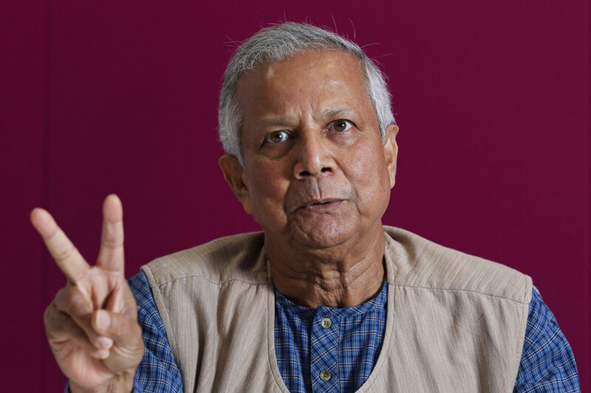
\includegraphics[scale=0.2]{figuras/yunus-final}
\label{figuraf}
\end{figure}

\end{frame}

\section{appendix}
	\begin{frame}{appendix 1}
	\justifying
{\small
\textbf{Normal p – variada: $N_p (\mu,\Omega)$.}
\begin{align}
f_x(x)= 2\pi^{-\dfrac{p}{2}}\vert\Omega\vert^{-\dfrac{1}{2}} \ exp \ \lbrace-\dfrac{1}{2}(x-\mu)^{T}\Omega^{-1}(x-\mu)\rbrace.
\end{align}

\textbf{T de Student p – variada con $\nu$ grados de libertad: $t_p(\mu,\Omega,\nu)$.}
\begin{align}
f_x(x)= \dfrac{\Gamma[\dfrac{1}{2}(\nu+p)]}{\Gamma[\dfrac{\nu}{2}(\nu\pi)^{\dfrac{p}{2}}]}\vert\Omega\vert^{-\dfrac{1}{2}}\lbrace1+\dfrac{1}{\nu}(x-\mu)^{T}\Omega^{-1}(x-\mu)\rbrace^{-\dfrac{1}{2}(\nu+p)}.
\end{align}
\begin{flushright}
\cite{leal2023}
\end{flushright}}
\end{frame}

\section{Bibliography}
	\begin{frame}[allowframebreaks]{Bibliography}
	\bibliographystyle{apalike}
	\bibliography{biblio}	
	\end{frame}
\end{document}
